\subsection{Object Life cycle}
\begin{center}\textit{Describe the life cycle of an object instance in Java and how garbage collection works}\end{center}

\subsubsection{Procedural Programming} 
Procedural programming preceded object-oriented programming. Basically, the code was written line by line, like a recipe. The computer would execute the lines in the order they appeared in the program. There were constructs to jump from one place to another, called gotos. But very quickly a program like that can become quite complicated, and specially the gotos would make it very hard to follow. 

With many lines of code, the program becomes difficult to maintain. We can split the program into several files and import the pieces when compiling. That helps programmers to organize the data but also fulfills the need for the compiler to have all the pieces of the program available. It doesn't solve the problem of scope, though. In procedural programming the data is accessible to the entire program. There is no clear ownership of data.

Procedural programming also provided constructs called subroutines. They are blocks of code, collections of instructions. Subroutines have their own scope, but any data they need to access outside the subroutine is still exposed to the entire program.

\subsubsection{Java is an Object-Oriented Language.} In object-oriented languages, instead of having data and subroutines, we deal with objects that have data and behavior. With object-oriented programming we can easily model the real world. For example we can have an object of a dog that has data (color, breed) and behavior (barks, runs, drools). 

When developers write Java programs, they write classes. A class is like a blueprint of an object. It defines the object. A class becomes an object when we instantiate it, we create an instance of it. Objects live when the program is executing, at runtime.

With objects it is easy to encapsulate behavior and data. We can restrict access to the data to only the members inside of a class. Nobody outside the class can access the data, if we don't want to (and we shouldn't want to.) We can define methods, or functions, 	that provide indirect, controlled access to the data inside the class.

Organizing code becomes easier too, because each file can only have one  public class per file\cite{spec}. Since each class encapsulates one "thing" that has a well-defined interface determining its behaviors, the code becomes very logical.

Everything in Java is made of another object. Java provides the mother of all objects, called \texttt{Object}, from which any other class must be based on.

\subsubsection{Instantiating a class}
We create an object from a class with the Java keyword \texttt{new}. Before instantiation, the object doesn't exist. After instantiation it exists. Classes have a special method called a constructor. After creating the class the JVM calls the object's constructor. If you don't provide a constructor for your class, its parent constructor is called. The JVM climbs the class hierarchy until it finds  a constructor, eventually the \texttt{Object}'s constructor. The constructor is a place where you could initialize the object or start resources.\cite{nicholas}
\subsubsection{Strongly Referenced}
When the constructor has been called, the program has a strong reference to it.\cite{reference} It means you we access the non-private methods and data on it. It is usable by the program.
\begin{lstlisting}[language=Java]
Dog pepper = new Dog();
\end{lstlisting}
In the above example, \texttt{pepper} is the handle, or a reference, to the object. It is a strong reference (as opposed to a weak reference) because we can use it to do things with the \texttt{pepper} object:
\begin{lstlisting}[language=Java]
pepper.bark();
\end{lstlisting}
\begin{figure}[H]\centering % Using \begin{figure*} makes the figure take up the entire width of the page
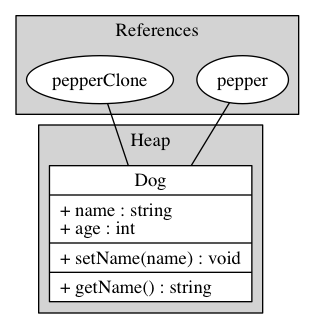
\includegraphics[width=0.5\linewidth, frame]{object-reference}
\caption{Object References}
\label{fig:object-references}
\end{figure}
\begin{figure*}[!htp]\centering % Using \begin{figure*} makes the figure take up the entire width of the page
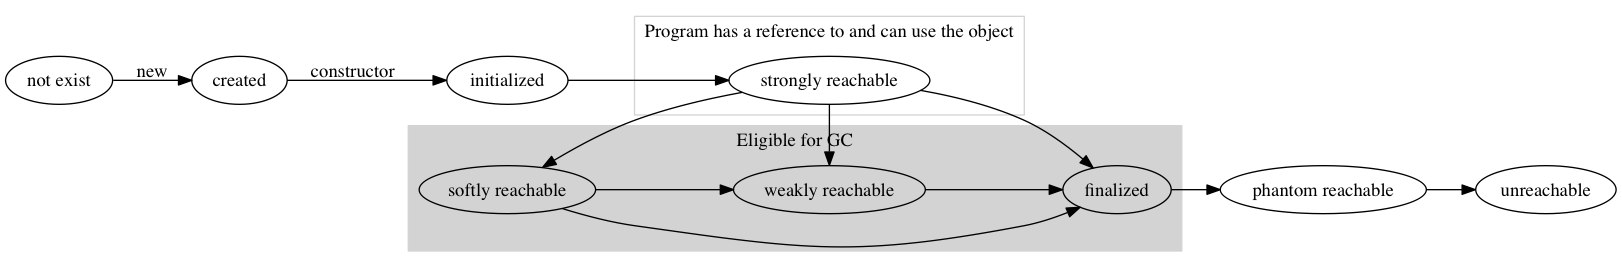
\includegraphics[width=\textwidth, frame]{object-life-cycle.png}
\caption{Object Life Cycle}
\label{fig:object-life-cycle}
\end{figure*}

We can have several references to the same object. Figure \ref{fig:object-references} on page \pageref{fig:object-references} shows two references, \texttt{pepper} and \texttt{pepper\hyp{}Clone} that point to the same object on the heap, of type Dog.

In listing \ref{lst:tworeferences} we create an instance of a \texttt{Dog} and get back a reference to it called \texttt{pepper} (line 2). Then we make \texttt{pepperClone} also point to the same object (line 5). After that we set the name of \texttt{pepper} to "pepper" (line 8). Because \texttt{pepper} and \texttt{pepper\hyp{}Clone} point to the exact same object, when we ask \texttt{pepperClone} for its name, we get "pepper" (line 13). 

\begin{lstlisting}[language=Java, caption=Multiple References to an Object, label=lst:tworeferences]
// create an instance of Dog
Dog pepper = new Dog();

// pepperClone also points to the same object
pepperClone = pepper;

// set pepper's name to "pepper"
pepper.setName("pepper");

// returns "pepper"
pepperClone.getName();

\end{lstlisting}
\vspace{2em}

Although it looks like we have two objects, we really are operating on one and the same object. We just have two references to it.

\subsubsection{Other references}
Once you let go of all the references to an object, it becomes eligible for garbage collection. The JVM still holds a weak or soft reference to the object (so it can manage it), but eventually, when it detects that memory needs to be cleaned up, it will finalize the object.\cite{reference}

Figure \ref{fig:object-life-cycle} on page \pageref{fig:object-life-cycle} shows all the states of an object lifecycle.
\begin{figure}[!h]\centering % Using \begin{figure*} makes the figure take up the entire width of the page
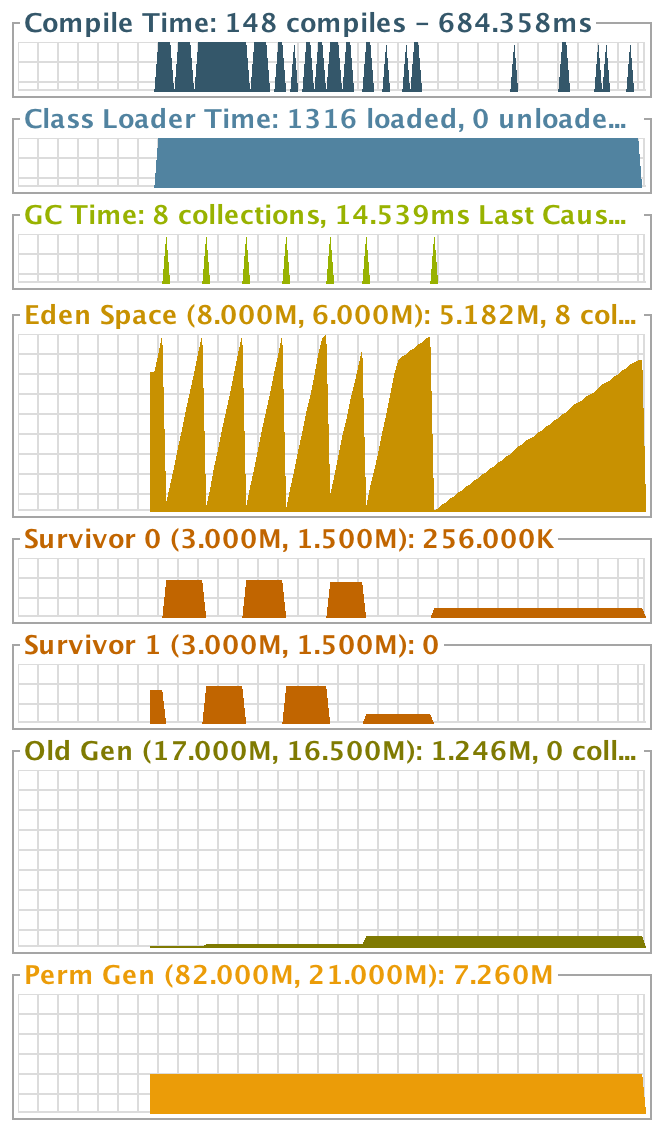
\includegraphics[width=\linewidth, frame]{garbage-collection}
\caption{Garbage Collection}
\label{fig:garbage-collection}
\end{figure}
\subsubsection{Garbage Collection.}
When the JVM determines that it needs to free memory, it will perform a garbage collection. The soft and weak references will be cleared before throwing an \texttt{Exception}.

Garbage collection is controlled by the JVM. We can tweak it to suggest a certain behavior to the garbage collector, and even suggest that it will do garbage collection (generally not a good idea), but eventually the garbage collector will decide when to run.

The benefit of garbage collection is that the programmer doesn't need to think about finalizing objects. When they are not needed, they may be thrown into garbage automatically.

There are times when this thinking can cause problems though. If we don't release the references the objects will never be garbage collected. An object is released when the program no longer holds a reference to it. For example, if we store objects in a collection that never goes out of scope, we still are holding a reference to the objects and they will not be collected. We can either set the reference to null or it will automatically be released when the object goes out of scope.

Figure \ref{fig:garbage-collection} shows garbage collection in action. Appendix A on page \pageref{App:AppendixA} links to a program (GarbageCollectionExample.java) that creates objects and puts them in a collection. With the visualvm tool provided in the Oracle JDK distribution we can vizualize the garbage collection\cite{garbagecollection}. The sample program creates 10,000 objects and then clears the collection. We create a total of 306,480,000 objects, and cleared the collection over 30,000 times. Garbage collection only kicked in 7 times, though. The heap size was set to 25MB. 

In the image we can also see the movement of objects from one generation to another.